\documentclass[11pt,a4paper]{article}
\usepackage[T1]{fontenc}\usepackage[utf8]{inputenc}\usepackage{lmodern,amsmath,amssymb,graphicx,booktabs,array,microtype,float,placeins,caption}
\usepackage[margin=25mm]{geometry}\usepackage[hidelinks]{hyperref}\usepackage{fancyhdr}
\pagestyle{fancy}\fancyhf{}\fancyhead[L]{Rooftop Photovoltaic Performance and Shading}\fancyfoot[C]{\thepage}\setlength{\headheight}{14pt}
\setlength{\parindent}{0pt}\setlength{\parskip}{6pt}\captionsetup{font=small,labelfont=bf}
\setlength{\emergencystretch}{2em}\begin{document}
\begin{titlepage}\centering\vspace*{25mm}
{\huge\bfseries Rooftop Photovoltaic Performance and Shading Analysis\par}\vspace{8mm}
{\Large TRNSYS and PVsyst Study for Tehran\par}\vspace{7mm}{\large Homework One\par}\vspace{20mm}
{\Large Pouya Asghari\par}\vspace{10mm}Renewable Energies Course\par Adviser: Dr. Pouria Ahmadi\par
\vfill School of Mechanical Engineering\par College of Engineering, University of Tehran\par
Original report date: 1404.08.03 (Iranian calendar)\par
\end{titlepage}
\section*{About this edition}
The supplied report is already in English. This edition converts it to editable LaTeX while retaining the narrative, equations, tables, numerical claims, and figures. Duplicate caption text and a leftover template instruction at the end of the abstract are removed. The original TRNSYS and PVsyst files, catalog, and exported PVsyst report are supplied unchanged alongside this report.

The historical narrative includes claims requiring qualification. In particular, the panel counts in the rooftop discussion differ from the exported PVsyst report, the monthly TRNSYS blocks use 720-hour periods, and the shadow-distance equations require consistent angle signs. A separate editorial appendix documents these issues. The simulations have not been rerun during preparation.
\begingroup\small\setlength{\parskip}{0pt}\tableofcontents\endgroup\clearpage


\FloatBarrier
\section{Abstract}

This work evaluates the performance and layout optimization of a VSUN450-144BMH photovoltaic module for rooftop deployment in Tehran. TRNSYS is used to model the I--V behavior at different irradiance levels and to simulate annual radiation, temperature, and PV power. PVsyst is then used to calculate minimum row spacing at winter solstice and to determine the maximum number of installable panels without shading losses. The results confirm the irradiance-dependence of PV output, the seasonal variability of power production, and a spacing-constrained upper limit on panel count enabling an optimized rooftop configuration.

\FloatBarrier
\section{Introduction}

The intensifying constraints on fossil fuel use and the associated environmental externalities have elevated the strategic relevance of solar photovoltaic (PV) technology within modern energy systems. PV generation is modular, fuel-free, and deployable in both centralized plants and distributed rooftops, offering a viable pathway toward decarbonized electricity supply.

PV modules convert incident solar radiation into electrical power via the photovoltaic effect, with performance governed by irradiance, temperature, and geometric exposure. In rooftop deployments, additional constraints arise from self-shading and limited installation area, making the joint evaluation of electrical behavior and spatial layout essential to design.

The present study aims to characterize the electrical response and annual production of the VSUN450-144BMH module for a rooftop in Tehran and to determine the maximum shading-free installation density. TRNSYS is used to model I--V curves and annual PV power, while PVsyst is used to compute winter-solstice spacing limits and the corresponding maximum deployable panel count.

\FloatBarrier
\section{TRNSYS Analysis}

The transient behavior of the system was analyzed using TRNSYS software. This study investigates how variations in daily meteorological conditions in Tehran - including ambient temperature, solar irradiance, and sky diffusivity - influence the electrical output of the selected photovoltaic module.

\subsection{Part A Current Voltage Curves}

For this part we want to find the IV curves of the system for different powers and compare it with the manufacturer’s catalogue.

\subsubsection{Design}

A new project was initially created in TRNSYS. For part (a), a calculator component was configured to supply the required input parameters to the photovoltaic modules. The time variable was converted into the corresponding input voltage through a simple division operation (1).

\begin{equation}V_{\mathrm{input}}=\mathrm{time}/100.\end{equation}

The simulation time step was adjusted to 1 hour, with the final simulation time set to 5000, corresponding to the reference I-V curve in the manufacturer’s catalogue, which has a maximum voltage of 50 V. Subsequently, the photovoltaic modules (Type103a) were configured. In the “Parameter” tab, module specifications were entered based on the catalogue data. For the “Input” tab, standard values were assigned to all variables, while the beam radiation was set to 1000 W/m\textsuperscript{2} to enable the plotting of the I-V curve. The module was duplicated twice, resulting in a total of three modules, with beam radiation values adjusted to 800 W/m\textsuperscript{2} and 600 W/m\textsuperscript{2}, respectively. The calculator component supplying the input voltages was then linked to each module. An online plotter (Type65c) was added to visualize the I-V curves, receiving the output current and power from all three modules. The plotter was configured with three axes to accommodate the three modules, with a maximum current of 20 A and a maximum power of 600 W. The simulation was then executed to generate the plots, which were compared with the manufacturer’s catalogue data.

\begin{figure}[H]\centering

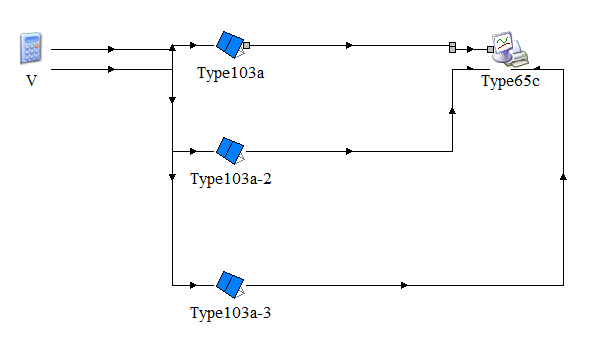
\includegraphics[width=0.94\linewidth,height=0.32\textheight,keepaspectratio]{figures/rId6.png}\par

\caption{TRNSYS schematic for the current--voltage sweep.}\end{figure}

\subsubsection{Comparison}

The plotted results reveal a discrepancy in the maximum power between the TRNSYS simulation and the manufacturer’s catalogue. This difference may arise from inaccuracies in the input parameters or from incomplete information provided to the modules. Nevertheless, the relative offset among the three curves closely matches that reported in the catalogue. Similarly, the current curves exhibit an approximate 5 A offset, likely attributable to the same sources of error.

\begin{figure}[H]\centering

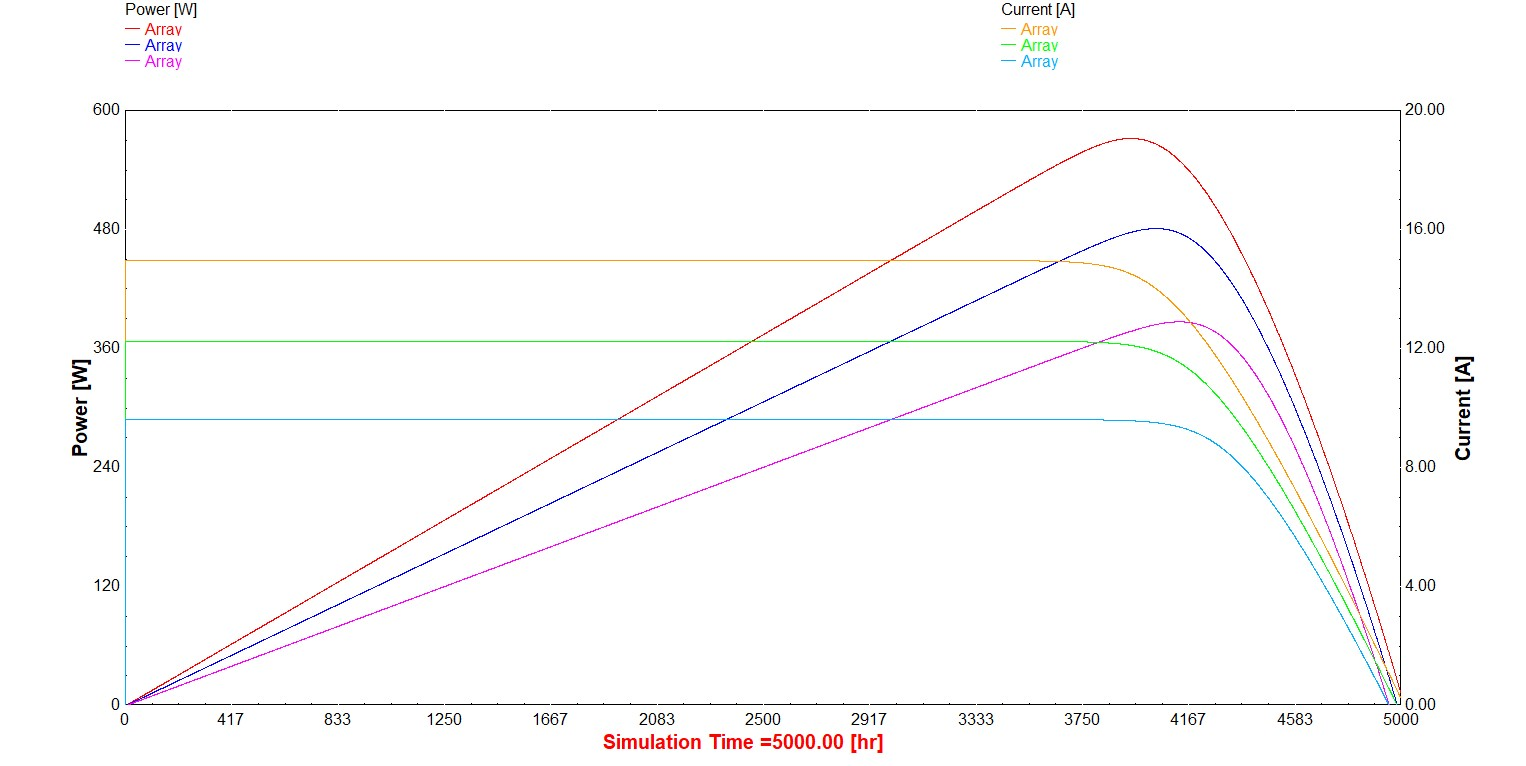
\includegraphics[width=0.94\linewidth,height=0.32\textheight,keepaspectratio]{figures/rId7.png}\par

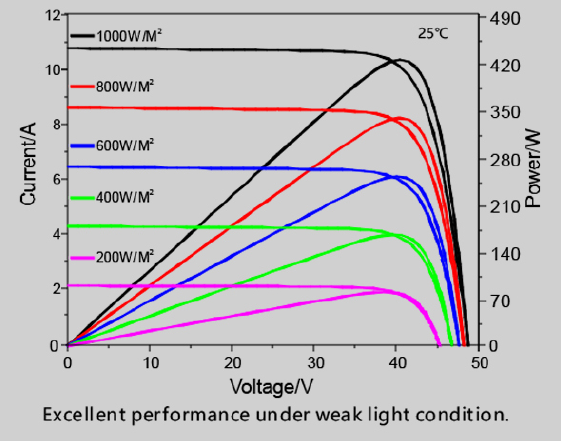
\includegraphics[width=0.94\linewidth,height=0.32\textheight,keepaspectratio]{figures/rId8.png}\par

\caption{TRNSYS electrical curves and catalog comparison.}\end{figure}

\subsection{Part B Annual and Monthly Performance}

This section investigates the annual variations in ambient temperature, solar radiation, and photovoltaic power output in Tehran. Subsequently, the study examines how the monthly power production of the PV system fluctuates throughout the year.

\subsubsection{Design}

For this analysis, weather data for Tehran was obtained from the Meteonorm database. A TMY2 file containing the relevant data was added to the workspace, and Tehran’s weather dataset was selected via the “External Files” tab. The simulation time step and final time were then defined. To plot the annual variations in temperature and solar radiation, the final time was set to 8,760 hours, corresponding to 365 days, and the time step was set to 1 hour to balance plotting efficiency with data resolution. Temperature data could be directly linked to the plotter, as it is expressed in $^\circ$C. In contrast, solar radiation required unit conversion, since the weather data is provided in kJ/(hr·m\textsuperscript{2}) whereas the plotter requires W/m\textsuperscript{2}. A calculator component was inserted between the weather data and the plotter to perform this conversion, following Equation (2).

\begin{equation}G=E_{\mathrm{in}}\frac{1000}{3600}.\end{equation}

For the weather data outputs, “Dry Bulb Temperature” was selected for the temperature plot, and “Total Tilted Surface Radiation” was chosen for the radiation plot. The left axis was assigned to radiation, while the right axis was designated for temperature. The plot boundaries were defined as follows: a temperature range of --10 $^\circ$C to 50 $^\circ$C and a maximum radiation of 1,200 W/m\textsuperscript{2}. With these settings, the simulation was prepared for calculation.

\begin{figure}[H]\centering

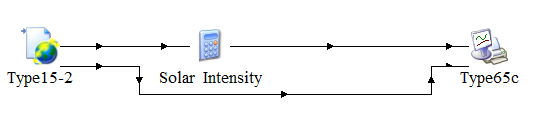
\includegraphics[width=0.94\linewidth,height=0.32\textheight,keepaspectratio]{figures/rId11.png}\par

\caption{TRNSYS schematic for ambient temperature and radiation.}\end{figure}

For the photovoltaic power analysis, the relevant weather data were provided as inputs to the PV module, following the configuration illustrated in the accompanying figure. Module parameters remained consistent with those used in previous sections. The array power output was linked to the plotter, with the maximum value set to 450 W.

To determine the monthly average power production, an integrator module was employed to sum the hourly power outputs over each month, followed by a calculator module to divide these sums by 720 hours (the approximate number of hours in a month). This procedure yielded 12 average values corresponding to each month of the year. The resulting monthly average power was then plotted and tabulated to visualize the temporal distribution of PV generation.

\begin{figure}[H]\centering

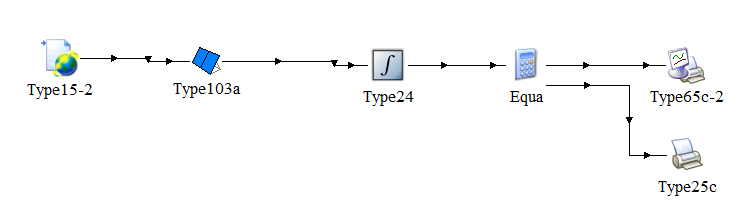
\includegraphics[width=0.94\linewidth,height=0.32\textheight,keepaspectratio]{figures/rId12.png}\par

\caption{TRNSYS schematic for period-average PV power.}\end{figure}

\subsubsection{Analysis}

The results indicate that the maximum ambient temperature in Tehran reaches approximately 41 $^\circ$C in June, while the minimum temperature falls to --7.5 $^\circ$C in January. Solar radiation peaks in June at roughly 1,080 W/m\textsuperscript{2}, whereas the lowest average radiation occurs in December, which necessitates calculating the optimal tilt angle for the PV modules under these conditions. The longest shadows are observed on December 21st, the date used for the simulations.

\begin{figure}[H]\centering

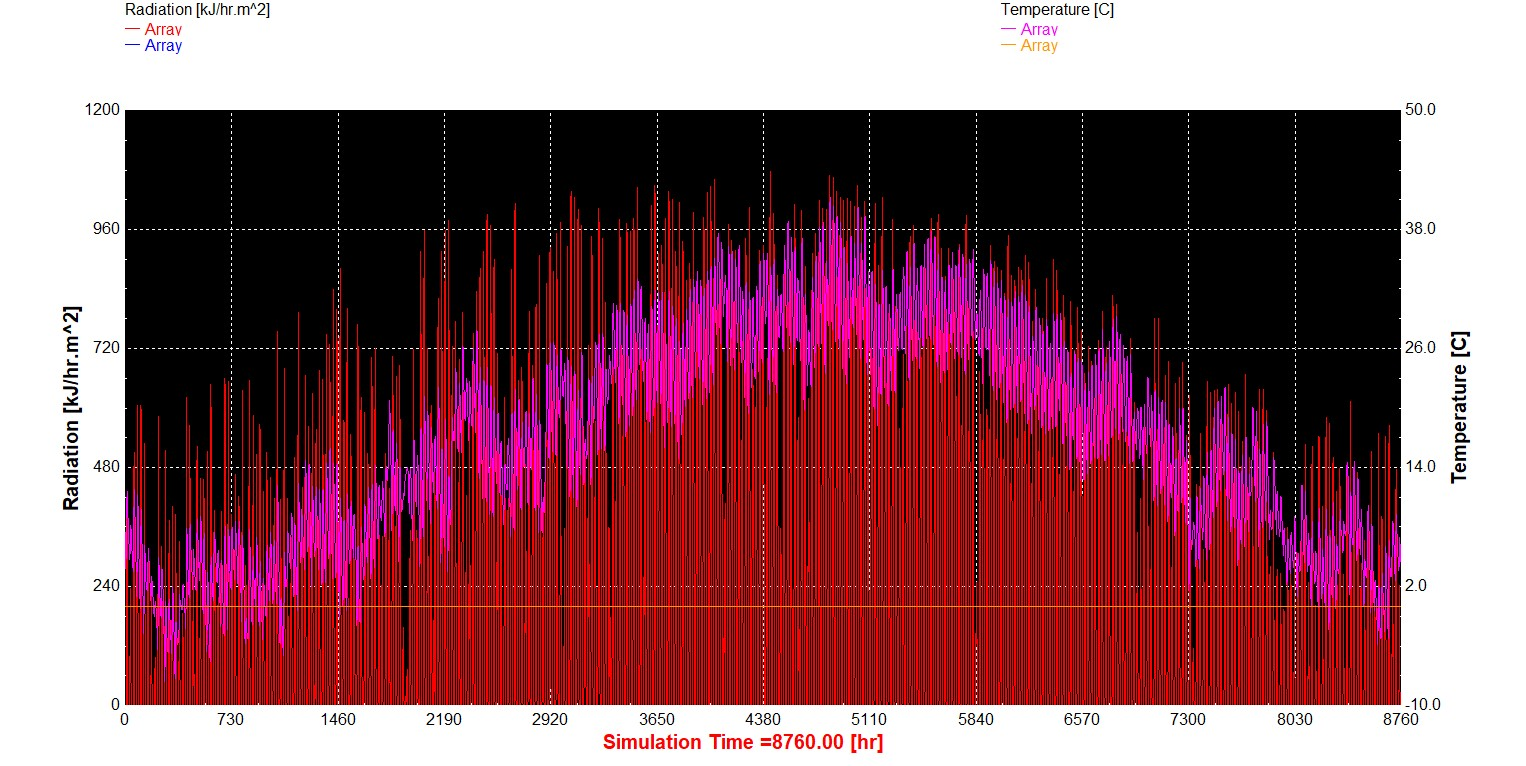
\includegraphics[width=0.94\linewidth,height=0.32\textheight,keepaspectratio]{figures/rId13.png}\par

\caption{Annual temperature and radiation plots.}\end{figure}

Regarding photovoltaic power output, the maximum occurs in June, reaching 405 W, while the minimum is observed in December at 90 W. The monthly average power production exhibits a bell-shaped curve, with a peak of approximately 128 W in June.

\begin{figure}[H]\centering

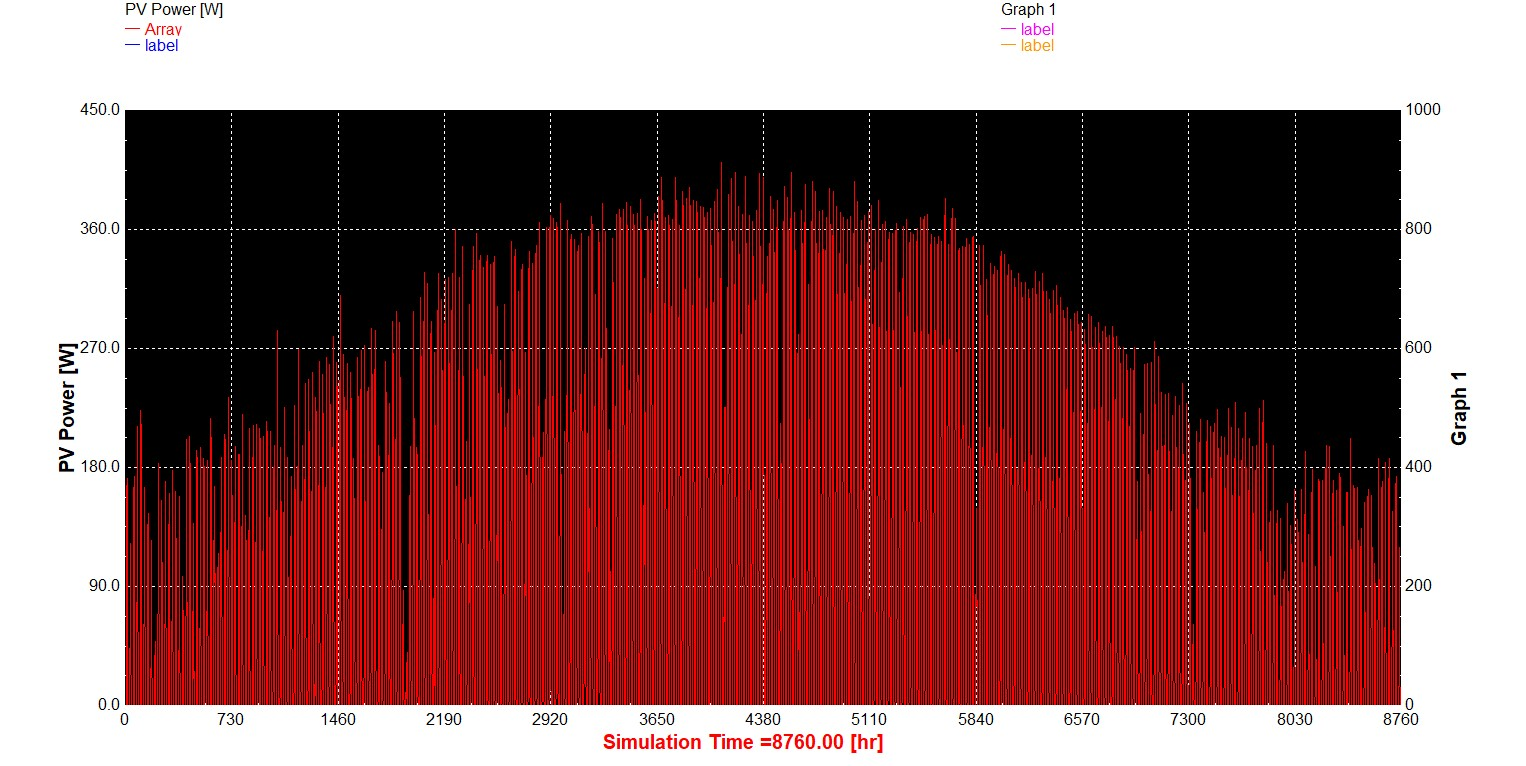
\includegraphics[width=0.94\linewidth,height=0.32\textheight,keepaspectratio]{figures/rId14.png}\par

\caption{Annual photovoltaic power plot.}\end{figure}

\begin{figure}[H]\centering

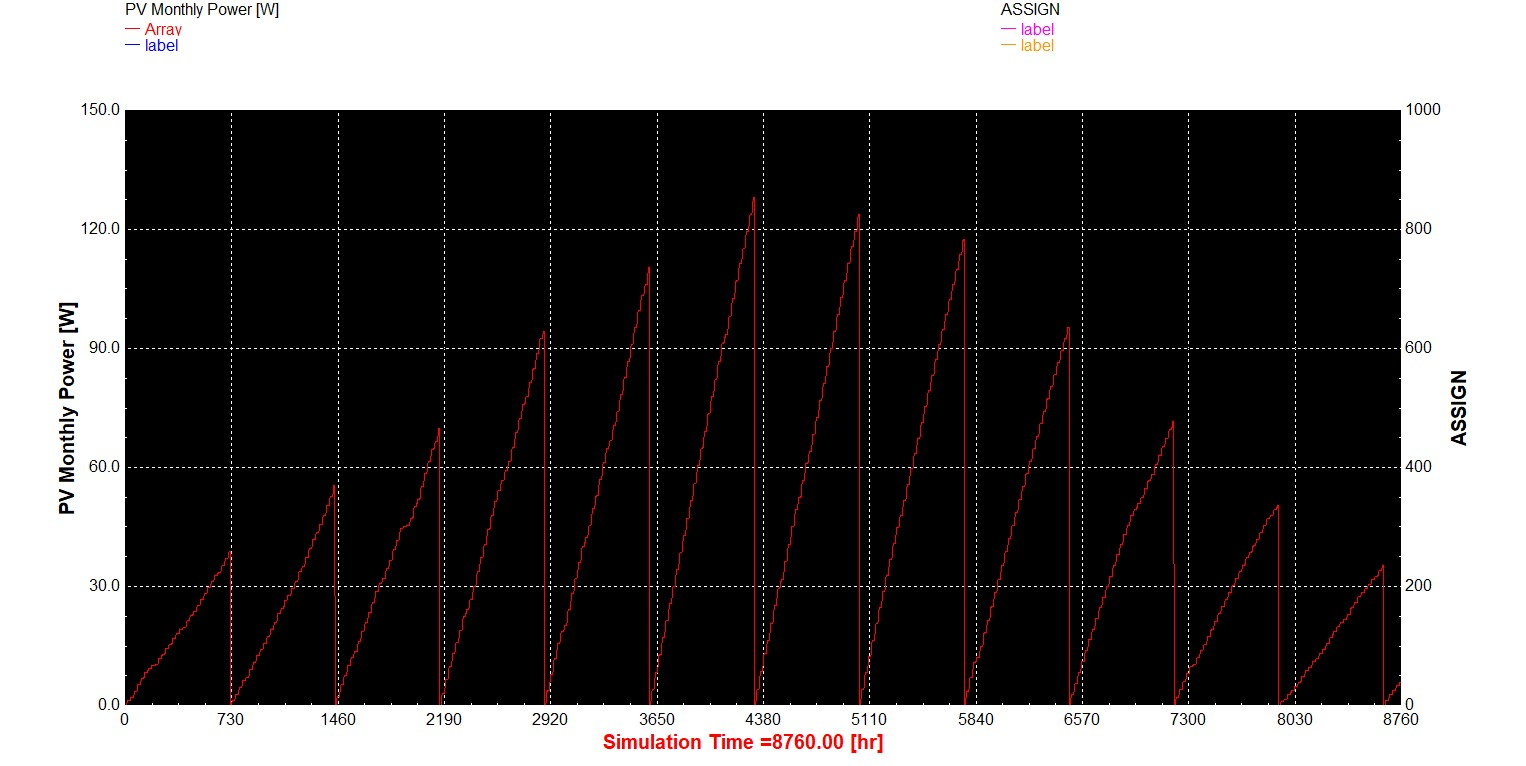
\includegraphics[width=0.94\linewidth,height=0.32\textheight,keepaspectratio]{figures/rId15.png}\par

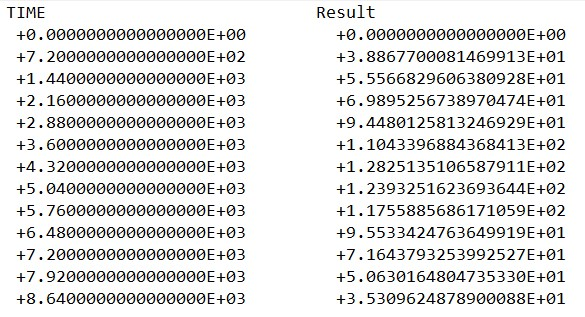
\includegraphics[width=0.94\linewidth,height=0.32\textheight,keepaspectratio]{figures/rId16.png}\par

\caption{Reported period-average power plot and numerical values.}\end{figure}

\FloatBarrier
\section{PVsyst Rooftop Layout}

This section focuses on designing the photovoltaic array and determining the optimal number of panels that can be installed on a given rooftop to maximize energy efficiency while minimizing beam losses.

\subsection{Part C Geometric Layout}

In this part, the number of photovoltaic panels is determined without the use of PVsyst. The following data were obtained from the manufacturer’s catalogue:

\begin{table}[H]\centering\caption{Module dimensions transcribed from the source.}\begin{tabular}{lr}\toprule Dimension & Value\\\midrule Length & 2108 mm\\Width & 1048 mm\\Thickness & 35 mm\\\bottomrule\end{tabular}\end{table}

\subsubsection{Calculations}

The solar angles were determined using the online tool available at \href{https://andrewmarsh.com/apps/staging/sunpath3d.html}{the Sun-Path 3D tool}, with the location set to Tehran and the date to the winter solstice, December 21st. The time was specified as 3:00 PM, representing the period with the longest shadows, which constitutes the worst-case scenario for system design. The resulting values obtained from the tool are as follows:

\begin{table}[H]\centering\caption{Solar and site angles reported in the source.}\begin{tabular}{lr}\toprule Quantity & Value\\\midrule Azimuth $\gamma$ & $-131.27^\circ$\\Altitude $\alpha$ & $12.45^\circ$\\Tehran latitude $\beta$ & $35.73^\circ$\\\bottomrule\end{tabular}\end{table}

Let L represent the width of a single panel, which is 1,048 mm. The minimum spacing between two consecutive rows of panels was calculated using equation (3):

\begin{equation}D_{\min}=\frac{L\sin\beta\cos\gamma}{\tan\alpha}=\frac{1.048\sin35.73^\circ\cos(-131.27^\circ)}{\tan12.45^\circ}=1.84\ \mathrm{m}.\end{equation}

The edge clearance for the photovoltaic panels was determined to be 18 in (457 mm) [1]. The rooftop layout indicates the presence of an object that casts significant shadows. To minimize shading effects, the minimum distance between the panels and this object was calculated. In this case, the height of the object (1 m) was used in place of L×sin($\beta$), which corresponds to the vertical dimension of the panels. Applying this adjustment yields the following equation (4):

\begin{equation}D_{\min,\mathrm{obj}}=\frac{h\cos\gamma}{\tan\alpha}=2.99\ \mathrm{m}.\end{equation}

It is important to note that Tehran is located in the Northern Hemisphere, which requires the photovoltaic panels to be oriented southward. Consequently, the resulting shadows predominantly extend to the north. Therefore, it is unnecessary to assume a circular exclusion zone around the obstructing object; a rectangular area is sufficient to avoid placing panels in shaded regions. The vertical height of each panel is given by L×cos($\beta$)=0.85 m, which is used for the top-view layout arrangement.

\subsubsection{Panel Arrangement}

As previously noted, a margin from the edges of the rooftop must be maintained. By adhering to all design constraints, a total of 17 panels can be installed, although this does not represent the optimal configuration. As illustrated below, all restricted areas have been avoided, and all panels are oriented southward. The panels are spaced 1.84 m apart and positioned 0.5 m from the edges of the rooftop.

\begin{figure}[H]\centering

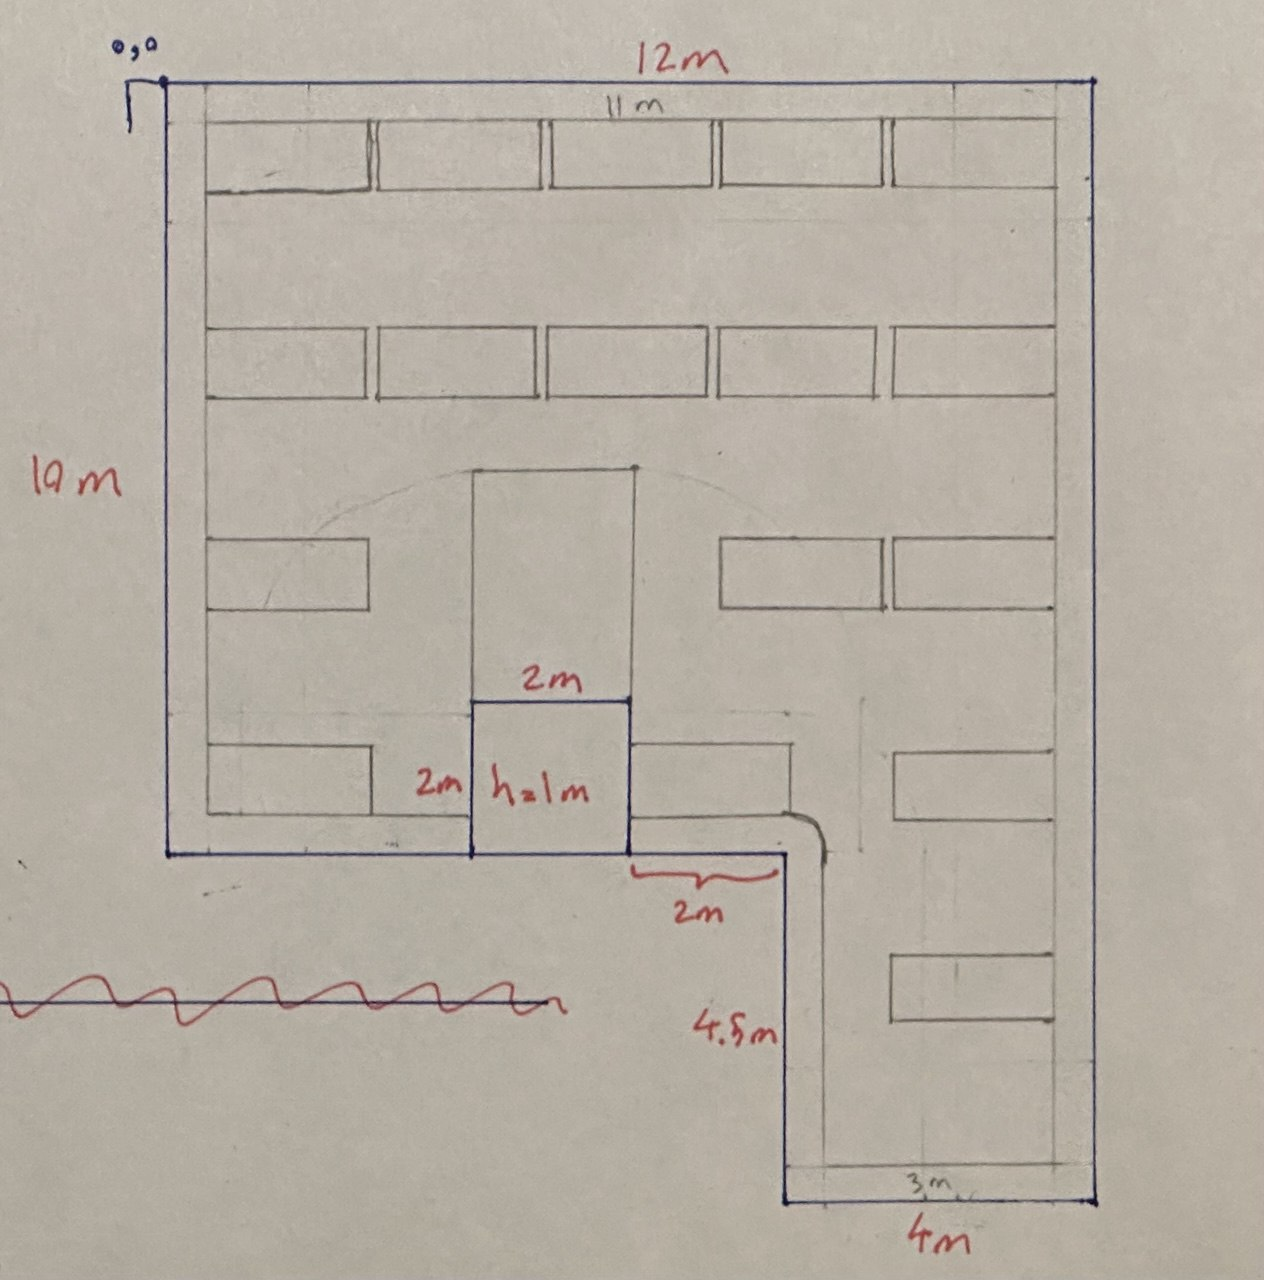
\includegraphics[width=0.94\linewidth,height=0.32\textheight,keepaspectratio]{figures/rId20.png}\par

\caption{Hand-drawn rooftop panel layout.}\end{figure}

\subsection{Part D PVsyst Model}

In this section, the previous analyses were replicated within the PVsyst environment. Additionally, the study examines the feasibility and efficiency of installing the panels in a vertical orientation.

\subsubsection{Design}

A new site was defined in PVsyst, specifying Tehran as the location and importing the annual weather data from Meteonorm. In the orientation settings, a tilt angle of 36$^\circ$ was selected. Within the system configuration, a planned power of 6 kWp was specified, with the PV module set to VSUN-450Wp35V-Simono-VSUN-450-144-MH and the inverter to Huawei 6 kW-90-560V. The “Use multi-MPPT feature” option was enabled. No errors were reported in the error box, indicating that the configuration is valid.

\begin{figure}[H]\centering

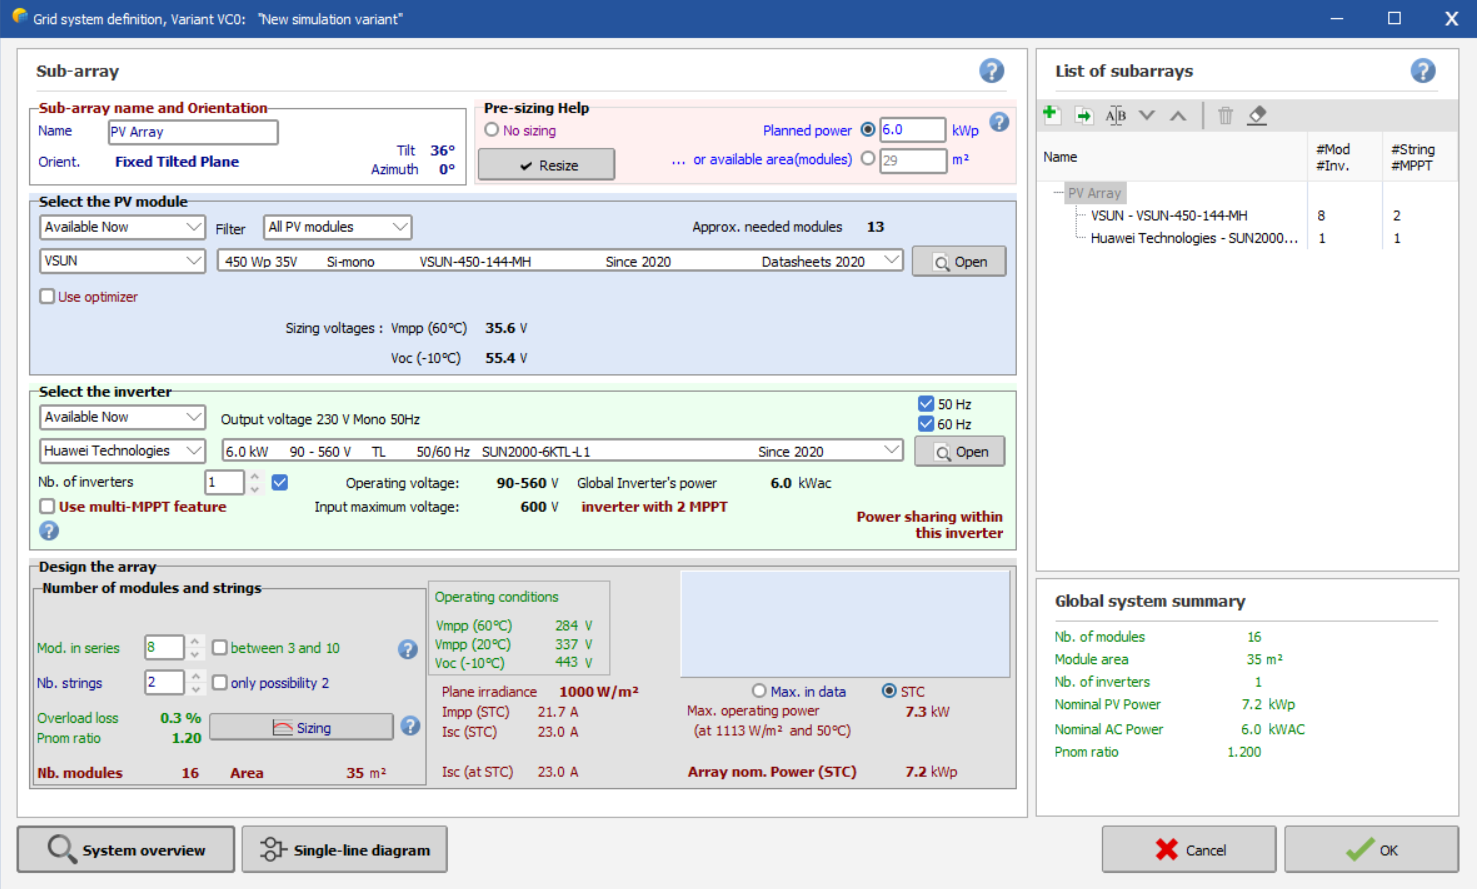
\includegraphics[width=0.94\linewidth,height=0.32\textheight,keepaspectratio]{figures/rId21.png}\par

\caption{System configuration in PVsyst.}\end{figure}

The “Near Shading” window was then opened to construct the 3D scene. The tilt angle of the panels was aligned with the previously specified value. A construction ground with a height of 1 m was added to ensure that the panels were elevated above the rooftop surface. Additionally, a virtual wall was included for visual realism; it does not cast shadows and therefore does not affect the shading simulation. Using this configuration, 21 panels could be installed on the rooftop while minimizing beam losses. All spacing requirements, including edge margins, inter-panel distances, and clearance from the obstructing object, were maintained.

\begin{figure}[H]\centering

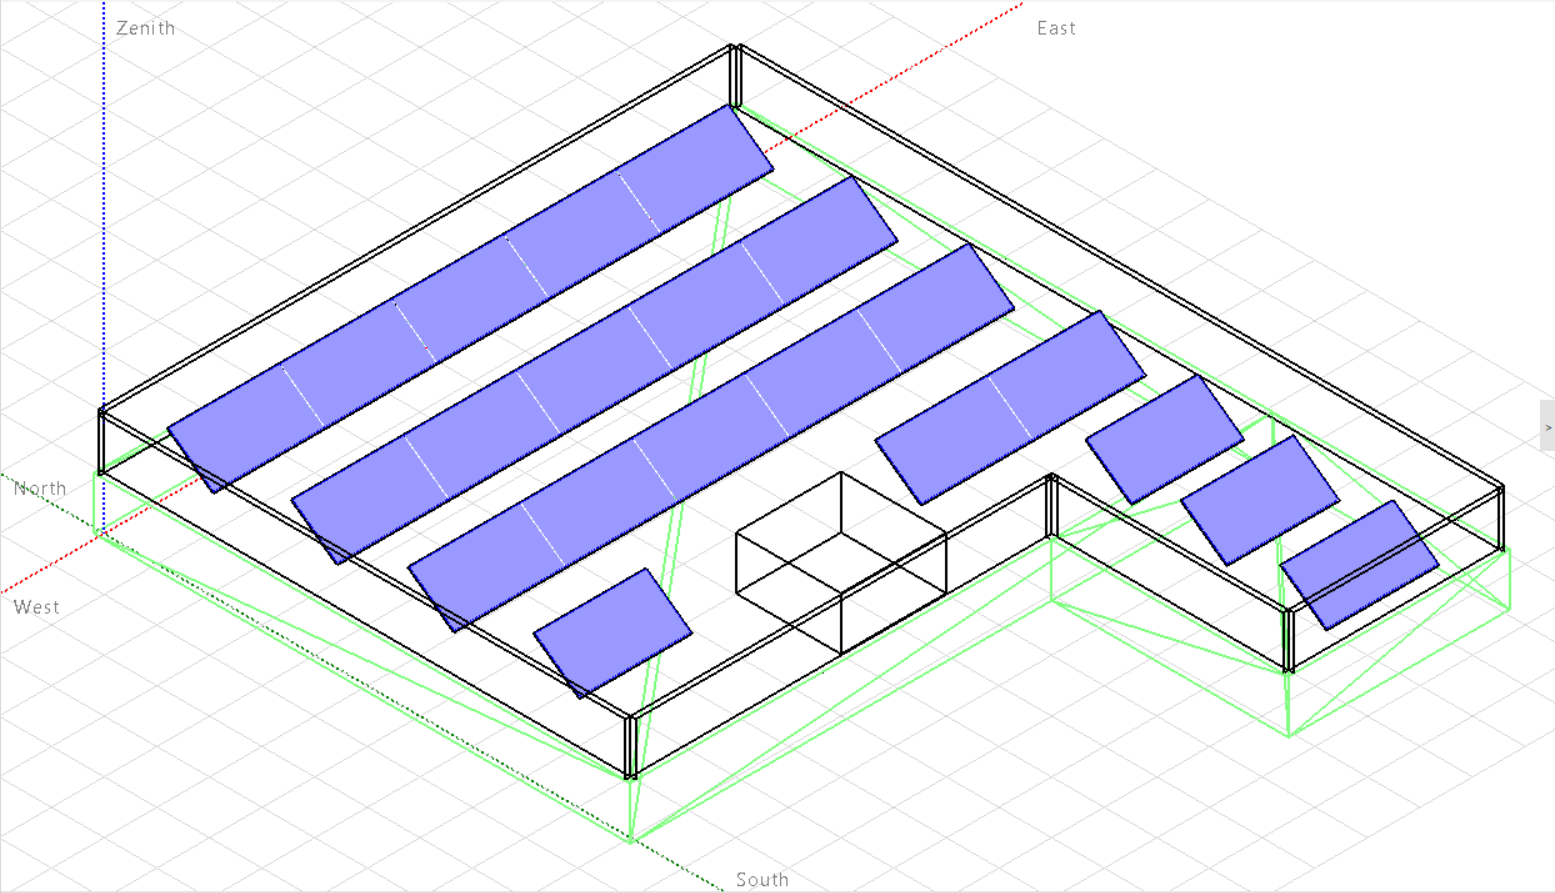
\includegraphics[width=0.94\linewidth,height=0.32\textheight,keepaspectratio]{figures/rId22.png}\par

\caption{PVsyst three-dimensional rooftop scene.}\end{figure}

Simulation results indicate that no shading occurs between 9:00 AM and 3:00 PM, which is desirable for optimal energy production. The arrangement could be further optimized by reducing the number of panels; however, this would also decrease the system’s maximum power output. Alternatively, a combination of landscape and portrait panel orientations could be employed to maximize the utilization of the available rooftop area.

\begin{figure}[H]\centering

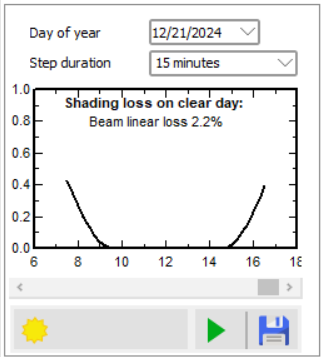
\includegraphics[width=0.94\linewidth,height=0.32\textheight,keepaspectratio]{figures/rId23.png}\par

\caption{Clear-day shading plot.}\end{figure}

The exported report from the PVsyst simulation is provided as an attachment.

\begin{figure}[H]\centering

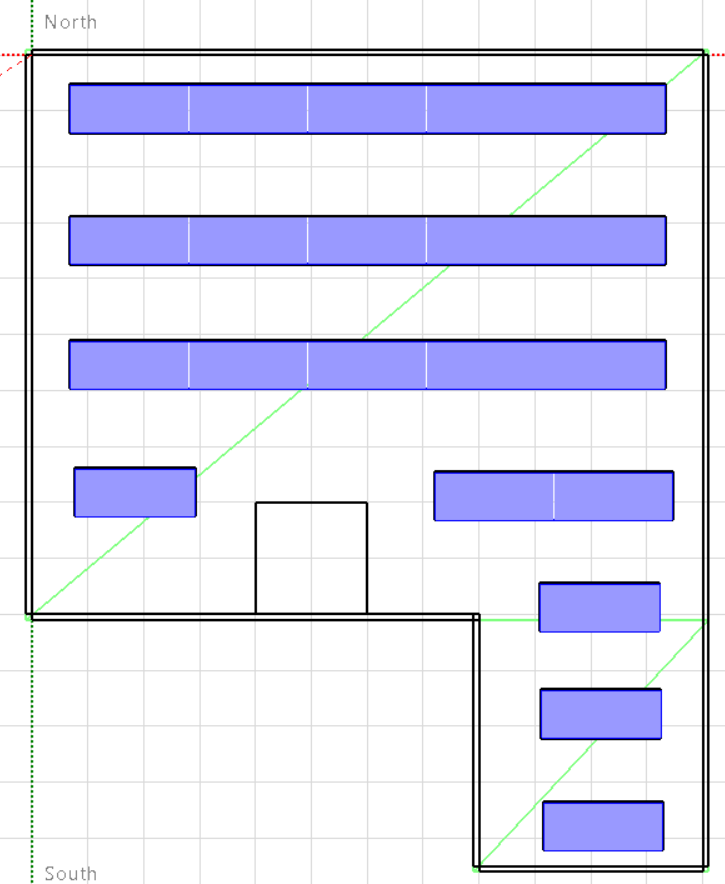
\includegraphics[width=0.94\linewidth,height=0.32\textheight,keepaspectratio]{figures/rId24.png}\par

\caption{Top view of the three-dimensional scene.}\end{figure}

\subsection{Portrait and Landscape Arrangement}

Utilizing a combination of landscape and portrait panels can significantly enhance system efficiency and reduce shading losses. For instance, instead of three rows of five landscape panels, two rows of ten portrait panels can be installed, adding five additional panels without introducing shading. The remaining panels are maintained in the landscape orientation, as this configuration is more suitable for their placement.

\begin{figure}[H]\centering

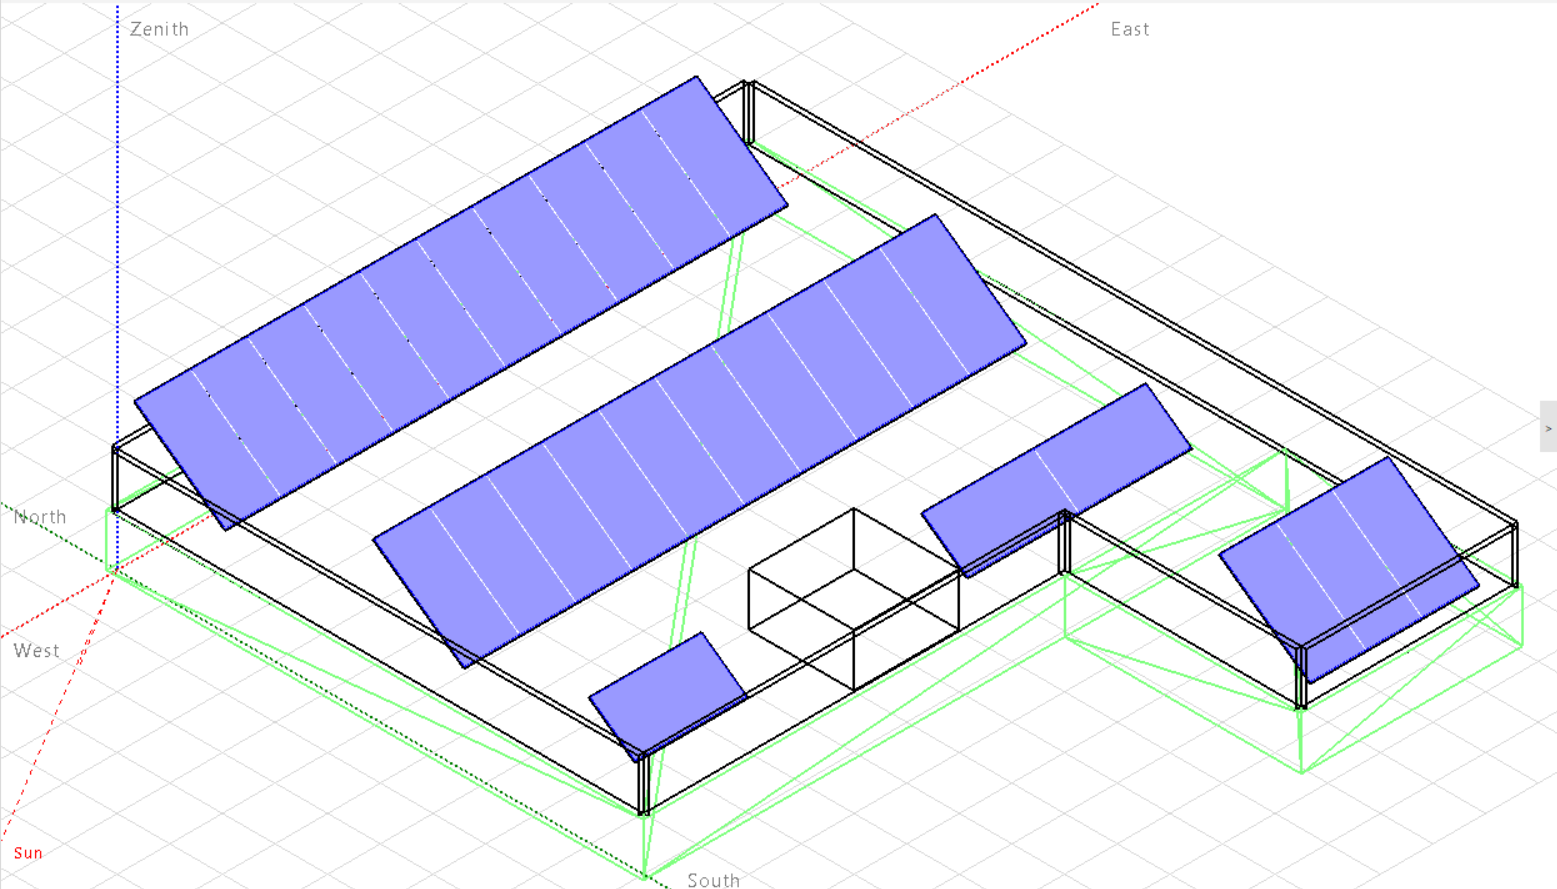
\includegraphics[width=0.94\linewidth,height=0.32\textheight,keepaspectratio]{figures/rId25.png}\par

\caption{Combined portrait and landscape layout.}\end{figure}

The results indicate that shading losses are reduced when the combined landscape and portrait panel arrangement is implemented.

\begin{figure}[H]\centering

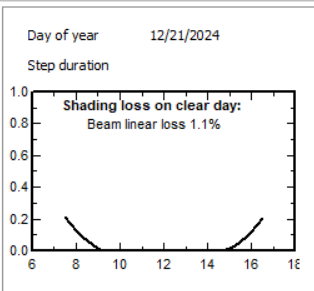
\includegraphics[width=0.94\linewidth,height=0.32\textheight,keepaspectratio]{figures/rId26.png}\par

\caption{Clear-day shading plot for the combined layout.}\end{figure}

\FloatBarrier
\section{Results and Discussion}

The study employed TRNSYS and PVsyst software to analyze the performance of a photovoltaic (PV) system installed in Tehran. Initially, TRNSYS was used to evaluate the transient behavior of the system, considering daily variations in ambient temperature, solar irradiance, and sky diffusivity. The I--V characteristics of the selected PV module were obtained for multiple power levels and compared with the manufacturer’s catalogue. Minor discrepancies were observed in maximum power and current values, likely due to input uncertainties or incomplete panel specifications. Despite these differences, the relative offsets among the curves closely matched the reference data, confirming the reliability of the simulation approach.

Subsequently, the annual variations of temperature, radiation, and PV power output were analyzed using hourly Meteonorm weather data. The results indicated that the maximum temperature in Tehran reaches approximately 41 $^\circ$C in June, while the minimum falls to --7.5 $^\circ$C in January. Solar radiation peaks at around 1,080 W/m\textsuperscript{2} in June and is lowest in December, necessitating adjustments in panel tilt angles for optimal performance. The PV power output correspondingly reaches a maximum of 405 W in June and a minimum of 90 W in December. Monthly average power production exhibits a bell-shaped distribution, with a peak of 128 W in June.

For rooftop design, panel spacing and orientation were optimized to minimize shading losses. Using geometric calculations based on panel dimensions and solar angles, the minimum spacing between rows and clearance from obstacles were determined. A total of 17 panels were initially fitted while adhering to all design constraints, including edge margins and shadowing considerations. Recognizing that Tehran is in the Northern Hemisphere, panels were oriented southward, with shadows extending northward.

Further simulations in PVsyst allowed for a detailed 3D assessment of shading effects. By constructing the rooftop scene, including ground elevation and virtual walls, it was possible to fit 21 panels with minimal beam loss. Simulation results confirmed that no shading occurred between 9:00 AM and 3:00 PM, indicating effective panel placement. Additional optimizations considered combining landscape and portrait panel orientations, which increased the number of panels and further reduced shading losses without compromising efficiency.

The accuracy of the simulations is supported by the close alignment between TRNSYS I--V curves and the manufacturer’s catalogue, as well as the realistic shading predictions from PVsyst. These results provide valuable insights for optimizing PV installations in urban environments. By improving panel placement and orientation, energy production can be maximized while minimizing losses, contributing to more sustainable and efficient use of rooftop spaces. This approach can inform future solar energy projects, supporting the broader adoption of renewable energy and helping reduce dependence on fossil fuels.

\FloatBarrier
\section{Original Reference}

\href{https://www.nfpa.org/news-blogs-and-articles/blogs/2024/02/29/residential-solar-panel-requirements}{NFPA residential solar panel requirements article (source URL).}

\FloatBarrier\clearpage\appendix\section{Editorial Review and Reproducibility Notes}
This appendix is separate from the original report. No model files or historical simulation results have been changed.
\subsection{Panel counts and the exported PVsyst variant}
The body describes a 17-panel hand layout, a 21-panel three-dimensional layout, and a mixed-orientation alternative without a fully reconciled final total. The supplied eight-page PVsyst export instead describes 16 modules, arranged electrically as two strings of eight, totaling 7.20 kWp DC with one 6 kW AC Huawei SUN2000-6KTL-L1 inverter. It records a fixed tilt of $36^\circ$ and azimuth of $0^\circ$ in PVsyst's convention.

The exported variant reports 12420.28 kWh/year injected energy, a specific yield of 1725 kWh/kWp/year, and a performance ratio of 81.55\%. These are simulated values for the exported 16-module variant, not verified results for the 21-panel layout. Its loss diagram includes 2.38\% annual near-shading irradiance loss. A source statement of no shading during selected clear-day hours is therefore not equivalent to zero annual shading loss. The report records PVsyst version 7.4.8 and Meteonorm 8.1 synthetic weather data.
\subsection{Shadow equations and conventions}
With the azimuth printed as $-131.27^\circ$, the cosine is negative, so the literal row-spacing expression in Equation (3) gives approximately $-1.84$ m, not the positive value printed in the source. The magnitude corresponds to the stated 1.84 m. A positive physical distance requires a consistent definition of the projected shadow direction and angle convention; do not silently use the source's sign as a validated layout rule. The same issue applies to the reported obstacle distance of 2.99 m.

The source calls $L\cos\beta$ a vertical height when discussing a top view; in that use it is the horizontal projected panel width. Latitude and selected module tilt are also different quantities even when a tilt close to latitude is adopted. A chosen winter-solstice afternoon time is a design check, not a proof of a globally worst shading condition for all objects and operating hours.

The report quotes an 18-inch edge-clearance value from a residential-solar reference. It is retained as a source design assumption, not established here as an applicable requirement for this Tehran roof. Site-specific access, structural, and installation requirements were not evaluated.
\subsection{TRNSYS time integration}
The monthly deck integrates over 720-hour periods and divides by 720 to produce average power. Twelve such periods cover 8640 hours, leaving 120 hours of a 8760-hour year outside those twelve equal blocks. These values are not exact Gregorian calendar-month means, and average power in watts is different from monthly energy in watt-hours or kilowatt-hours. The supplied \texttt{b\_PVmonthly} table reaches a maximum of approximately 128.251 W at 4320 hours under this convention.
\subsection{Electrical model checks}
The source acknowledges offsets between simulated and catalog current/power curves. Matching trends alone does not independently validate the module model. The saved monthly power deck contains a series cell count of 36 and module area of 2.21 square meters. Confirm the intended module electrical representation and the units of the temperature coefficients against the supplied catalog and component documentation before relying on the outputs. The TRNSYS module named in the report and the PVsyst database model have different recorded identifiers, so their equivalence should also be checked.
\subsection{Files and external dependencies}
Native TRNSYS decks, Simulation Studio projects, parameter files, logs, listings, saved plot/output files, screenshots, both PVsyst project ZIPs, the module catalog, and the original PVsyst report are included in the repository. Each PVsyst ZIP contains a project file, a variant file, and Meteonorm-derived weather data. Both contain identical internal filenames and should be restored separately to avoid accidental overwrites. The labels portrait and landscape come from the original archive filenames; the variants have not been imported and compared in PVsyst during conversion.

The TRNSYS decks reference absolute Windows paths, including the Tehran TMY2 file and output locations. The referenced TMY2 file is not included as a standalone dependency. The MET file inside a PVsyst backup is not a direct substitute for the TRNSYS TMY2 file. Update data and output paths in working copies using compatible local resources. Check component availability and application versions before attempting a new run.

The original report is in English and was converted rather than translated. Figures and native files remain unchanged. Additional separately stored scripts can be added with their actual language, dependencies, and run commands. No missing code or rerun validation is claimed.
\end{document}